
\noindent 1. (\textbf{CLRS 15.2-1}) Determine a parentização ótima de um produto de cadeia de matrizes cuja sequência de dimensões é $\langle 5, 10, 3, 12, 5, 50, 6 \rangle$.\\[6pt]
\textbf{Resposta:} Como a sequência tem 7 elementos, o valor de $n = 6$. A figura \ref{fig:6.1-1} mostra cada iteração da entrada para geração da matriz $m$ que contém o número mínimo de multiplicações escalares necessário para calcular o produto $A_1..A_n$.

\begin{center}
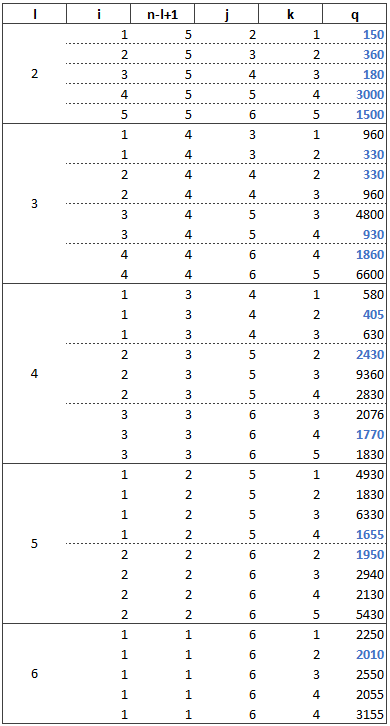
\includegraphics[width=0.6\textwidth]{q6-1-p1.png}
\captionof{figure}{Cálculo do número mínimo de multiplicações escalares}
\label{fig:6.1-1}
\end{center}

Os valores destacados em azul são aqueles menores para uma dada iteração $i, j$ e, consequentemente, são armazenados na matriz $m[i, j]$, como pode ser visto na figura \ref{fig:6.1-2}.
\begin{center}
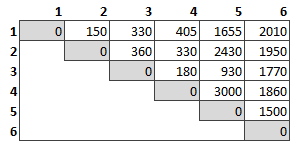
\includegraphics[width=0.4\textwidth]{q6-1-p2.png}
\captionof{figure}{Matriz $m$ preenchida após todas as iterações}
\label{fig:6.1-2}
\end{center}

A figura \ref{fig:6.1-3} mostra uma segunda matriz $s$ utilizada para armazenar o valor de $k$, de forma que possamos rastrear a sequência ótima para multiplicação posteriormente.
\begin{center}
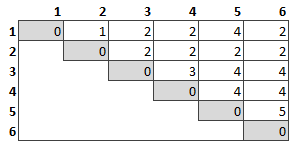
\includegraphics[width=0.4\textwidth]{q6-1-p3.png}
\captionof{figure}{Cálculo do número mínimo de multiplicações escalares}
\label{fig:6.1-3}
\end{center}

Sendo assim, a sequência ótima é $( (A_1 A_2) ((A_3 A_4) (A_5 A_6)) )$.\\[12pt]